\section{Block-Encodings}
\label{sec:block-encoding}

Quantum algorithms are constructed as a series of unitary operators.
However, it is often necessary to apply non-unitary operators within a quantum algorithm.
Block-Encoding refers to an access model to non-unitary operators wherein the information regarding the operator is stored in a labeled subspace of a larger unitary operator.

If we let $A$ represent some $2^{N_A}\times2^{N_A}$ non-unitary operator then a block-encoding of $A$ is given by:
\begin{equation}
    U_A = 
    \begin{pmatrix}
    \bar{A} & * \\
    * & * 
    \end{pmatrix}
\end{equation}
where $U_A$ is the larger unitary operator, $\bar{A}$ is a rescaled form of the original operator such that $||\bar{A}|| \leq 1$, and matrix entries $*$ denote matrix elements that are restricted such that the $U_A$ is unitary.

The action of the block-encoding on an arbitrary quantum state ($\ket{\psi}$) can be defined as:
\begin{equation}
    \label{eq:general-block-encoding}
    U_A \ket{\psi} \ket{0}_{\text{anc}} = \bar{A} \ket{\psi} \ket{0}_{\text{anc}} + \beta_\psi \ket{\perp}
\end{equation}
where $\ket{}_{\text{anc}}$ is the ancilla register used to produce the block-encoding, $\beta_\psi$ is a complex coefficient that normalizes the quantum state and is dependent on the initial state of the system register.

The dependence of $\beta$ on $\ket{\psi}$ can be seen in a simple case where $\ket{\psi}$ is an eigenstate of $\bar{A}$.
Let $\ket{\lambda_k}$ be an eigenstate of $\bar{A}$ with eigenvalue $|k| < 1$.
In this scenario, Eq. \ref{eq:general-block-encoding} becomes:
\begin{equation}
    U_A \ket{\lambda_k} \ket{0}_{\text{anc}} = k \ket{\lambda_k} \ket{0}_{\text{anc}} + \sqrt{1 - |k|^2} \ket{\perp}
\end{equation}
where $\sqrt{1 - |k|^2}$ is clearly dependent upon the eigenstate.
One could also generalize this to the case of non-eigenstates using the spectral decomposition of $\ket{\psi}$ in the eigenbasis of $\bar{A}$.

In the above equations, the encoded subspace of $U_A$ is chosen (without loss of generality) to be the all-zero state of the ancilla register.
The portion of the state of both the system and ancilla register given by $\ket{\perp}$ represents the branch of the wavefunction that is outside of the encoded subspace.
This portion of the state can typically be disregarded, but it is orthogonal to any quantum state with nonzero amplitude of the ancilla register in the all-zero state.

We can interpret the action of the block-encoding as a probabilistic application of $\bar{A}$.
If we apply the block-encoding followed by a measurement of the ancillae register, then a measurement result that corresponds to the encoded subspace (an all-zero measurement result) implies that $\bar{A}$ has been applied to the quantum state.

The rescaling that is applied to $A$ is often referred to as the rescaling factor:
\begin{equation}
    A = \lambda \bar{A}
\end{equation}
This rescaling factor can have important implications in the cost of quantum algorithms, though the exact impact on the cost is algorithm-dependent.
For example, the success probability of applying $\bar{A}$ as described above is a function of the rescaling factor.
For a fixed operator $A$, the success probability descreases as the rescaling factor increases. \ws{explicitly define this relationship.}
If the block-encoding is used in Quantum Phase Estimation as is done in \cite{poulin2018quantum, babbush2018encoding, lee2021even}, then the output estimates correspond to the rescaled operator and the rescaling factor must be accounted for in postprocessing.

One might notice that there is not a single $\bar{A}$ for each $A$ as the only restriction is that the spectral norm satisfies $|\bar{A}| \leq 1$.
To motivate why smaller rescaling factors are typically more favorable, consider the case that $|\bar{A}| = 1$.
This implies that there exists at least one eigenstate $\ket{\lambda}$ such that applying the block-encoding onto the eigenstate results in the state: $U_A \ket{\lambda}\ket{0}_{\text{anc}} = \bar{A} \ket{\lambda}\ket{0}_{\text{anc}} = \ket{\lambda}\ket{0}_{\text{anc}}$.
In other words, the output state after the block-encoding is applied remains \textit{entirely} within the encoded subspace.

In the following subsections, we will describe two commonly used frameworks for constructing block-encodings of different operators: the Sparse-Oracle framework and Linear Combination of Unitaries (LCU).
The Sparse-Oracle framework allows for constructing block-encodings of a more general class of operators, while LCU is restricted to operators described as a linear combination of unitary operators.
However, LCU block-encodings typically result in lower rescaling factors. 
In the final subsection, we discuss a framework for constructing block-encodings of linear combinations of operators that uses a similar structure to LCU to give similar rescaling factors.


\subsection{Sparse-Oracle Block-Encoding Framework}
\label{subsec:sparse-be}

The Sparse-Oracle framework for constructing block-encodings has been used to give algorithmic speedups or many applications such as Hamiltonian simulation \cite{berry2009black, childs2009universal, berry2015hamiltonian,berry2015simulating, low2017optimal,childs2017quantum,gilyen2019quantum}.
These works assume the presence of oracles that both the location of the nonzero matrix elements and the values of those elements.

Lin et. al \cite{lin2022lecture} defines three oracles ($D_s$, $O_A$, and $O_c$) to produce a Sparse-Oracle block-encoding as follows:
\begin{theorem}
    \label{th:sparse-oracles}
    Let $s$ represent the maximum number of nonzero entries in a single row of a matrix $A$ where each element of $A$ has magnitude at most $1$.
    Let $A_{ij}$ be the matrix element in the $i^\text{th}$ row and the $j^\text{th}$ column.
    Let $c(j, l)$ be a function that returns the row-index of the $l^\text{th}$ nonzero matrix element in the $j^\text{th}$ column.

    Define the oracle $D_s$ as:
    \begin{equation}
        \label{eq:diffusion}
        D_s \ket{0^n} = \frac{1}{\sqrt{s}} \sum_{l=0}^{s-1} \ket{l}
    \end{equation}
    where $D_s$ is the ``diffusion operator'' and $n \equiv \lceil \log_2{s} \rceil$.
    If $s$ is increased to the nearest power of $2$ by treating some zero-valued elements as nonzero, then $D_s$ is implemented by:
    \begin{equation}
        \label{eq:diffusion-had}
        D_s = H^{\otimes n}
    \end{equation}
    where $H$ is the Hadamard gate.

    Define the oracle $O_A$ as:
    \begin{equation}
        \label{eq:value-oracle}
        O_A \ket{0} \ket{j}\ket{i} = \big( A_{ij} \ket{0}  + \beta_{ij} \ket{1} \big) \ket{j}\ket{i}
    \end{equation}
    where $\beta_{ij} \equiv \sqrt{1 - |A_{ij}|^2}$.

    Finally, define the oracle $O_c$ as:
    \begin{equation}
        \label{eq:column-oracle}
        O_c \ket{j} \ket{l} = \ket{j}\ket{c(j, l)}
    \end{equation}

    Then a block-encoding for $A$ is given by:
    \begin{equation}
        \label{eq:so-be}
        U_A = D_s O_c O_A D_s
    \end{equation}
    with a rescaling factor of:
    \begin{equation}
        \lambda_\text{SO} = 2^n \max_{ij} {|A_{ij}|} 
    \end{equation}

\end{theorem}
A simple proof that $U_A$ block-encodes $A$ is given in Camps et. al \cite{camps2024explicit}.

For a matrix $A$, the factor of $2^n$ comes from the sparsity of the matrix and the factor $\max_{ij} {|A_{ij}|}$ comes from the constraint in Theorem \ref{th:sparse-oracles} that all elements of $A$ have magnitude at most $1$.
It is also worth noting that the factor of $2^n$ can be reduced to $s$ by simply replacing the diffusion operator with the generalized \textit{Uniform State Preparation} (USP) protocol which is discussed in Appendix \ref{sec:usp}.
Implementing USP is less time-efficient than the diffusion operator, so a trade-off exists between reducing the rescaling factor and reducing the number of non-transversal gate operations.
Since the impact of the rescaling factor on the spacetime cost is algorithm dependent, we simply note this alternative compilation choice but do not explore it in detail. 

Although these oracles - and the analogous oracles assumed in other works \cite{berry2009black, childs2009universal, berry2015hamiltonian, berry2015simulating,low2017optimal,childs2017quantum,gilyen2019quantum} - produce valid block-encodings, none of these works provide quantum circuits that implement these oracles.
In Camps et. al \cite{camps2024explicit}, a framework for constructing explicit quantum circuits for these oracles for general matrices ($D_s$, $O_A$, and $O_c$) is given.
From this, explicitly compiled Sparse-Oracle block-encodings of the form given in Eq. \ref{eq:so-be} can be generated and several works \cite{camps2022fable, liu2024efficient, sanavio2024explicit} \ws{add more citations here} have explored such compilations for particular systems. 

\subsubsection{Sparse-Oracles for Fermionic Pairing Hamiltonian}

Liu et. al \cite{liu2024efficient} use the framework proposed by Camps et. al \cite{camps2024explicit} to construct a Sparse-Oracle block-encoding for a pairing Hamiltonian of the form:
\begin{equation}
    \label{eq:pairing-ham}
    H = \sum_{ij}h_{ij}b^\dagger_i b_j
\end{equation}
where $b^\dagger$ and $b$ are the fermionic creation and annihilation operators respectively and an arbitrary ordering of these operators is imposed such that the terms are indexed by $l \in [0, L)$.

\begin{figure}[h]
    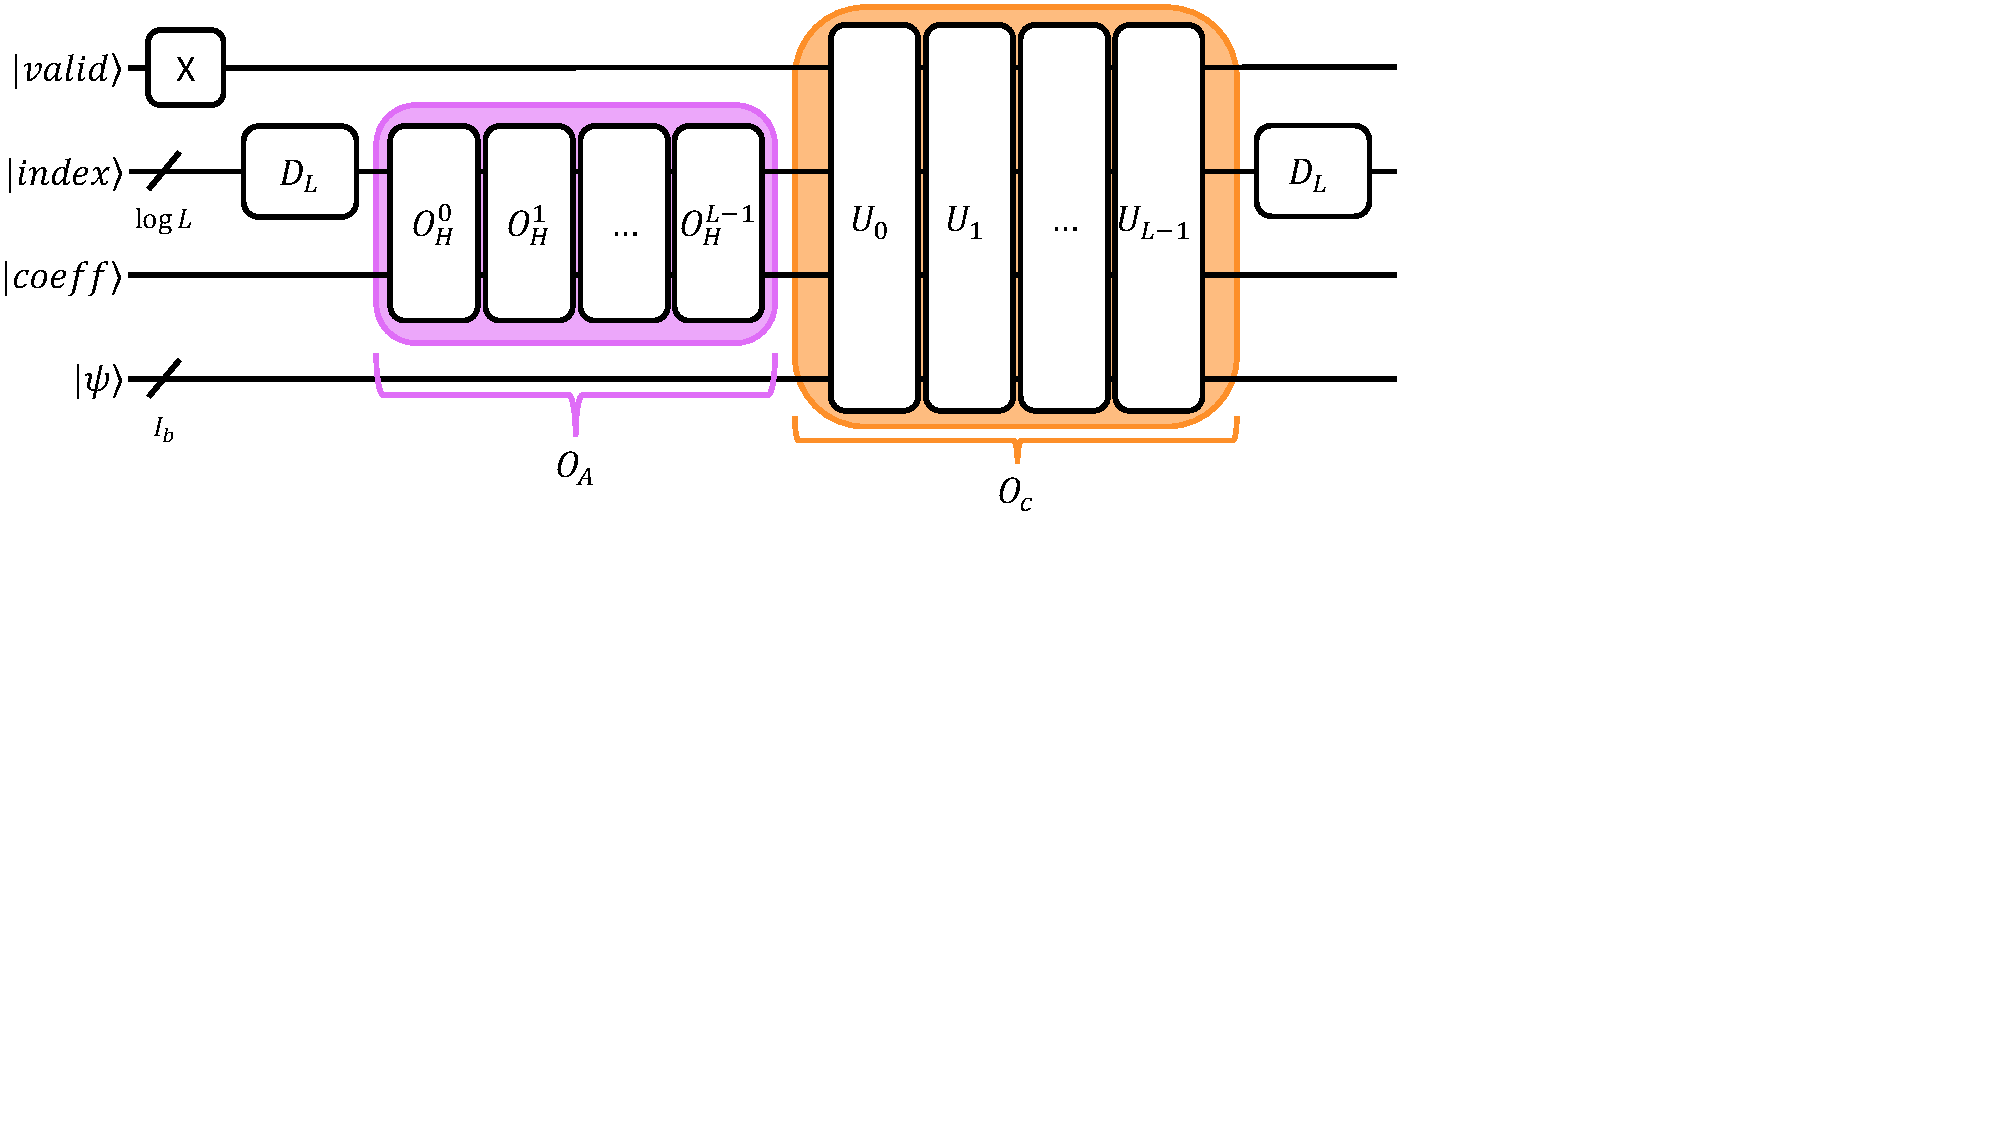
\includegraphics[width=12cm]{figures/liu-construction.pdf}
    \caption{
        \textbf{Sparse-Oracle Block-Encoding Circuit for Pairing Hamiltonians}
        A circuit diagram for the block-encoding described by Liu et. al \cite{liu2024efficient} is shown.
        The $O_A$ oracle is implemented by the series of $O_H^l$ operators (shaded in purple) which load the coefficients of the $l^{th}$ term.
        The $O_c$ oracle is implemented by the series of $U_l$ operators (shaded in orange) which apply the $l^{th}$ term onto the state.
        The $D_L$ oracle represents the diffusion operator (Eq. \ref{eq:diffusion-had}) acting on $L$ terms where $L$ is raised to the nearest power of two.
        The unitary $U_H = D_L O_c O_A D_L$ implements a block-encoding of the pairing Hamiltonian (Eq. \ref{eq:pairing-ham}) assuming the validation qubit ($\ket{\text{valid}}$) is initialized in the $\ket{1}$ state.
        The rescaling factor of this block encoding is given by $\lambda = L \max_{ij} {|h_{ij}|}$.
    }
    \label{fig:liu-construction}
\end{figure}

The structure of the circuits to block-encoding the pairing Hamiltonian is given in Figure \ref{fig:liu-construction}.
The sequence of $O_H^l$ unitaries implement the $O_A$ oracle and the sequence of $U_l$ unitaries implement the $O_c$ oracle.

\begin{figure}[h]
    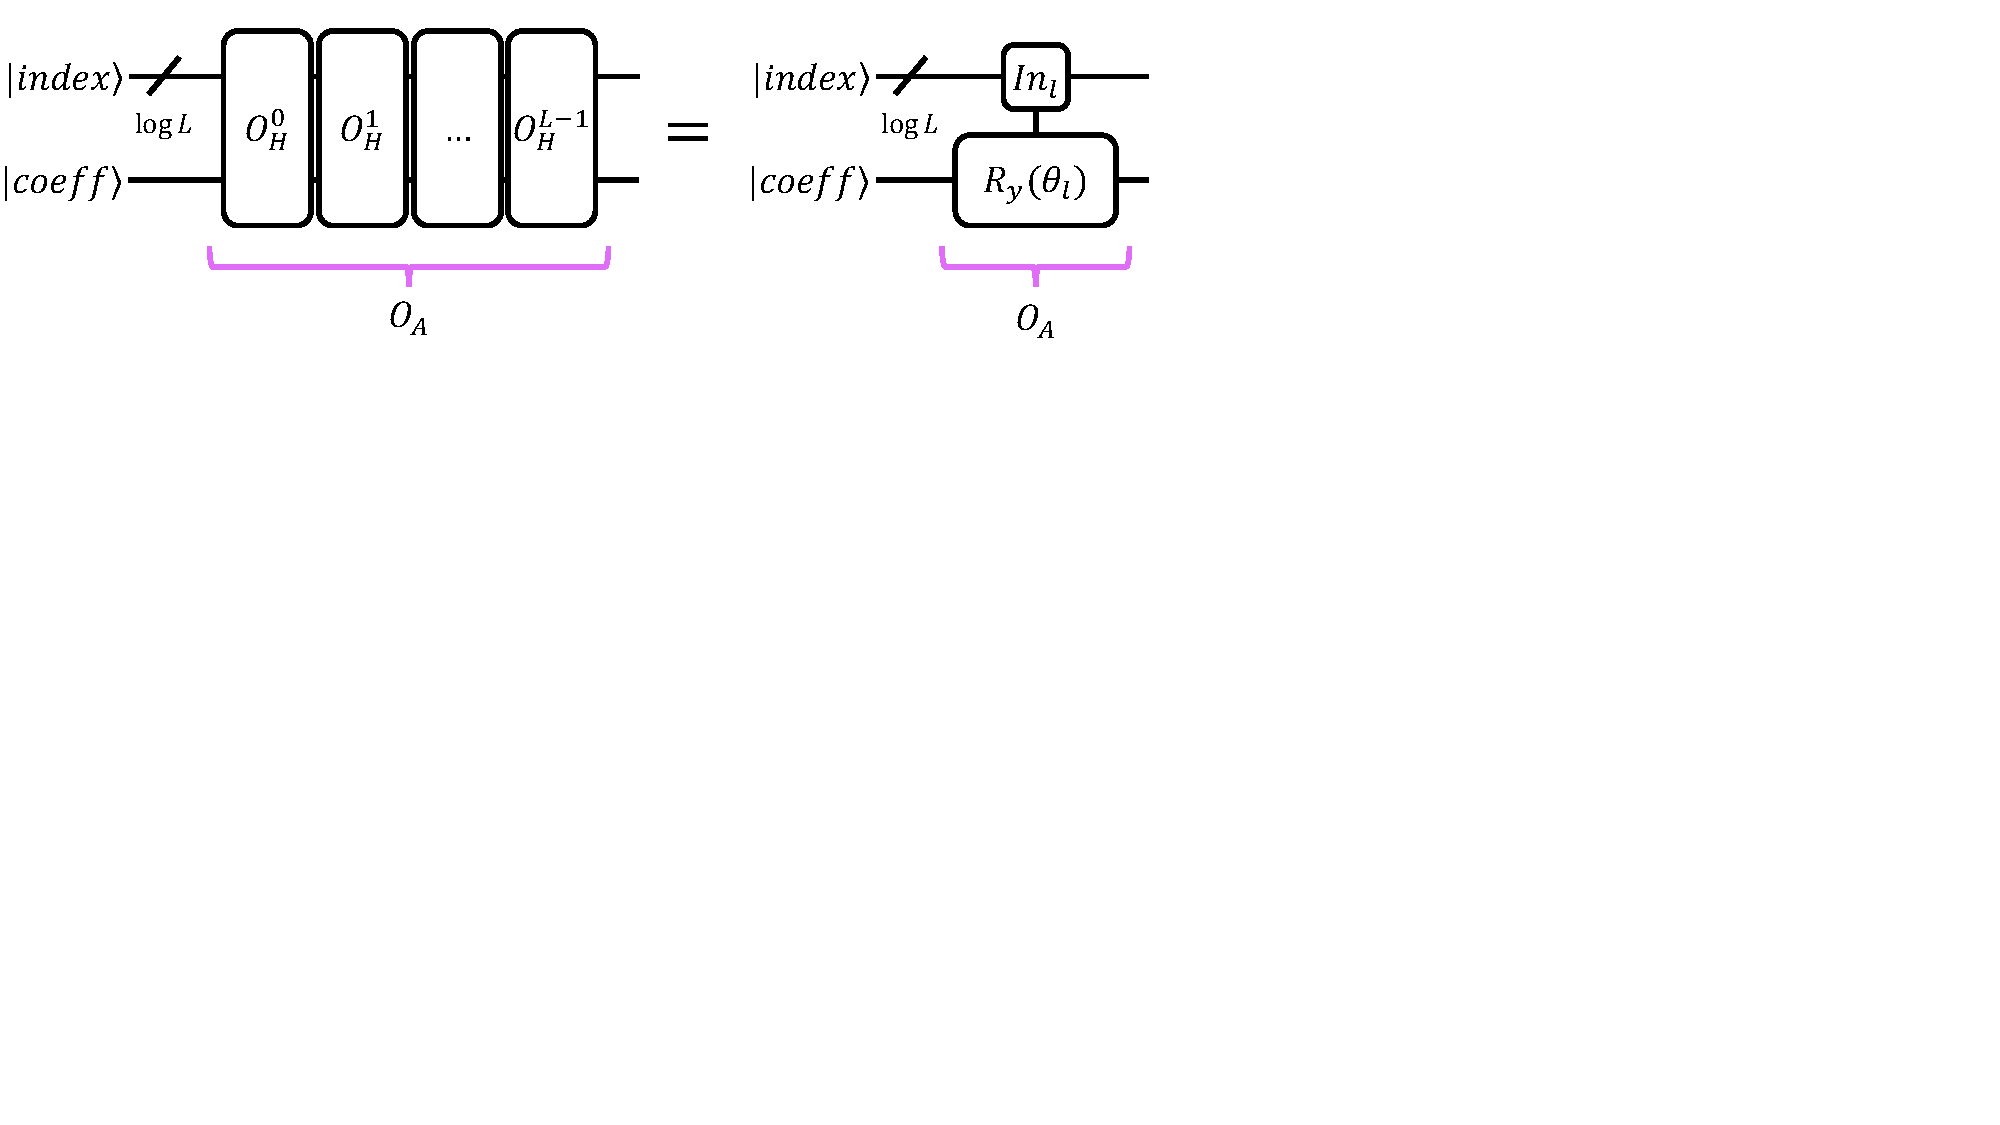
\includegraphics[width=12cm]{figures/liu-O_A.pdf}
    \caption{
        \textbf{$O_A$ Circuit for Pairing Hamiltonians}
        A circuit diagram for the $O_A$ oracle described by Liu et. al \cite{liu2024efficient}.
        Each unitary in the subfigure on the left performs an $R_y$ rotation on the coefficient qubit, controlled on the index register being in the computational basis state $\ket{l}$.
        This sequence of controlled rotations is referred to as a set of uniformly controlled rotations which is depicted by the subfigure on the right.
        Further discussion of compiling uniformly controlled rotations is given in Appendix \ref{sec:multiplexed-rotations}.
    }
    \label{fig:liu-O_A}
\end{figure}

Following Eq. \ref{eq:value-oracle}, the $O_A$ oracle rotates an ancilla qubit ($\ket{\text{coeff}}$ in Figure \ref{fig:liu-construction}) proportionally to the coefficient of the $l^\text{th}$ term when the index register ($\ket{\text{index}}$) is in the computational basis state $\ket{l}$.
This can be achieved by an $R_y$ rotation:
\begin{equation}
    \begin{split}
        & R_y (\theta_l) \ket{0}_\text{coeff} = h_{ij} \ket{0}_\text{coeff} + \sqrt{1 - |h_{ij}|^2} \ket{1}_\text{coeff} \\
        & \theta_l = 2 \cos^{-1}{(h_{ij})}
    \end{split}
\end{equation}
where the rotation is controlled on the index register being in the $l^\text{th}$ computational basis state.

This sequence of rotations controlled on the basis states of the index register is sometimes referred to as a set of uniformly controlled rotations.
When the axis of the rotations is the same for each rotation (as is the case here), the decomposition given by Möttönen et. al \cite{mottonen2004transformation} can be applied.
Under this construction, the $O_A$ oracle can be implemented using $L$ uncontrolled rotations.
A further discussion of this compilation is given in Appendix \ref{sec:multiplexed-rotations}.

The $O_c$ oracle is constructed by the unitaries denoted as $U_0 \dots U_{L - 1}$ in Figure \ref{fig:liu-construction}.
Each unitary $U_l$ is controlled on the index register being in the computational basis state $\ket{l}$.
This series of controlled operations can again be described as a set of uniformly controlled operations where each operation being applied is constructed to apply a block-encoding of the $l^\text{th}$ term in the Hamiltonian onto the system register.

\begin{figure}[h]
    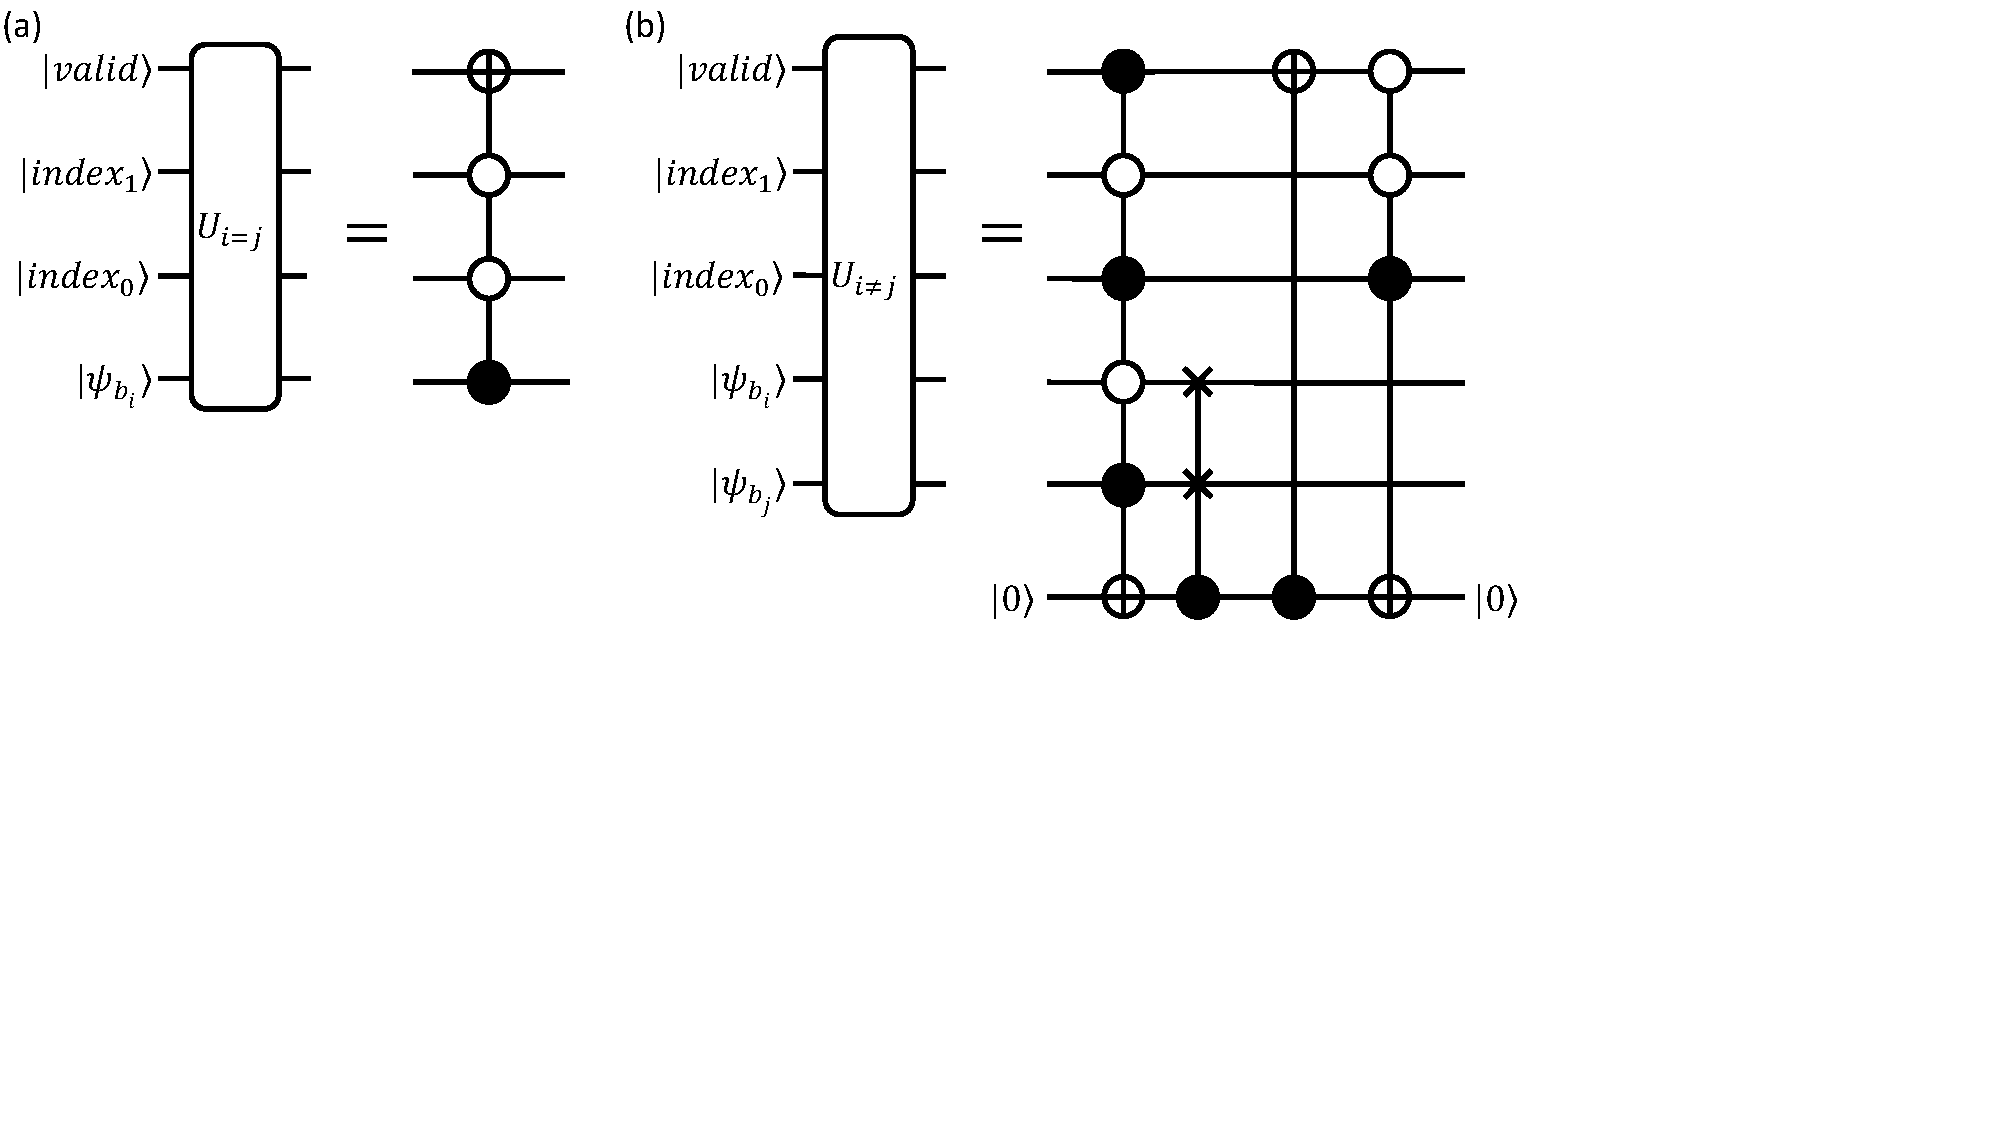
\includegraphics[width=12cm]{figures/liu-O_c.pdf}
    \caption{
        \textbf{$O_c$ Circuit Components for Pairing Hamiltonians}
        A circuit diagram for the unitaries comprising the $O_c$ oracle described by Liu et. al \cite{liu2024efficient} are shown.
        The circuit in subfigure a shows the unitary $U_{i = j}$ which applies a block-encoding of the operator $b_i^\dagger b_i$ when the index register is in the computational basis state $\ket{0}$. 
        The circuit in subfigure a shows the unitary $U_{i \neq j}$ which applies a block-encoding of the operator $b_i^\dagger b_j$ when the index register is in the computational basis state $\ket{1}$. 
    }
    \label{fig:liu-O_c}
\end{figure}

Liu et. al give constructions for applying the terms in the pairing Hamiltonian onto the system under the two cases $i = j$ and $i \neq j$.
In their construction, the validation qubit is initialized in the $\ket{1}$ state and is used to block-encode the individual terms in the Hamiltonian.

When the index for the ladder operators in Eq. \ref{eq:pairing-ham} are the same ($i = j$), the operator $b_i^\dagger b_i$ should zero-out the quantum state when the $i^\text{th}$ mode is unoccupied and should leave the state unchanged when the mode is occupied. 
For these terms, the desired action on the validation qubit is to leave it unaltered when the mode is unoccupied and flip the state of the validation qubit to $\ket{0}$ when the mode is occupied.
This can be achieved by a Toffoli gate which is controlled on the $i^\text{th}$ mode being occupied and the index register being in the computational basis state $\ket{l}$.
An example of these operators is given in Figure 11 of \cite{liu2024efficient} and we give a reproduction in Figure \ref{fig:liu-O_c}a.

When the indices that the ladder operators act on are not the same ($i \neq j$), the operator $b_i^\dagger b_j$ should zero-out the quantum state unless both the $i^\text{th}$ mode is unoccupied \textit{and} the $j^\text{th}$ mode is occupied.
Otherwise, the system of the state would be zeroed-out which would be indicated by leaving the validation qubit unchanged (in the $\ket{1}$ state).
If these conditions are true, a swap gate can be applied to swap the occupations of the fermionic modes and the validation qubit should be flipped to the $\ket{0}$ state. 

To perform this action, an ancillae qubit can be used to store the logical-AND of the conditions on the validation qubit, the index register, and the occupation states of the fermionic modes.
We assume that this ancilla qubit begins in the $\ket{0}$ state and the intent will be to return it to the $\ket{0}$ state such that it can be reused on subsequent operations.
In this work, we refer to qubits that are only temporarily rotated outside of the $\ket{0}$ state as clean ancillae.
An example for a circuit to perform this operation is also given in Figure 11 of \cite{liu2024efficient} and we give a reproduction in Figure \ref{fig:liu-O_c}b.
We note that to properly uncompute the ancilla qubit and return it to the $\ket{0}$ state we include the controls on the index register.
These controls are not present in the constructions given by Liu et. al, but must be included to properly reset this ancilla qubit.
\ws{Determine if construction by Liu et. al is actually incorrect or just incorrect if you want to treat the ancilla qubit as a clean ancilla.}

The controls on the index register for each $U_l$ comprising the $O_c$ oracle ensure that only the $l^\text{th}$ term is applied when the computational basis state is in the $\ket{l}$ state.
These controls on the index register are present for each term and can be accounted for by the uniformly controlled operation structure discussed in more detail in Appendix \ref{sec:uniformly-controlled-operations}.



\subsection{Linear Combination of Unitaries}
\label{subsec:lcu}

Suppose we wish to generate a block-encoding of an operator that can be written as a linear combination of unitary operators:
\begin{equation}
    \label{eq:lcu}
    A = \sum_{l=0}^{L-1} \alpha_l U_l
\end{equation}
where $\alpha_l$ are real-valued coefficients and each $U_l$ is a unitary operator.
The restriction here on real-valued coefficients is simply to be clear about the cost of block-encoding this operator. 
If we wish to include terms with imaginary coefficients, we can absorb the imaginary phase into the operator: $i \alpha_l U_l = \alpha_l U_l^\prime$.
Likewise, a term with a complex coefficient can be treated as two distinct terms ($U_l$ and $U_l^\prime$) each with a real coefficient, though this increases the number of terms ($L$).
\ws{Question: when we decompose a state into a linear combination of other states we say we expand it in some basis. What is the wording for when we expand an operator in a basis of operators?}

Assuming that $A$ is sparse in this description - $L$ grows polynomially with $N_A$ - then the Sparse-Oracle framework generates a valid block-encoding of $A$ where the rescaling factor would be $\lambda = 2^{\lceil \log_2 L \rceil} \max_{l} |\alpha_l|$.
In this construction, $O_A$ would load the (rescaled) coefficients $\{\alpha_l\}$ and $O_c$ would apply the unitaries $\{U_l\}$ onto the system register controlled on the index register being in the computational basis states $\{\ket{l}\}$. 

However, an alternative framework proposed by Childs et. al \cite{childs2012hamiltonian} called Linear Combination of Unitaries (LCU) is \textit{specifically} designed for generating block-encodings of operators in the form of Eq. \ref{eq:lcu}. 
With two oracles, \textit{Prepare} and \textit{Select}, an LCU block-encoding can be defined as follows:
\begin{theorem}
    \label{th:lcu}
    Given a matrix $A$ defined by Eq. \ref{eq:lcu}, let the oracles \textbf{Prepare} and \textbf{Select} be defined by:
    \begin{equation}
        \label{eq:prep-state}
        \textbf{Prepare}\text{:} \ket{0^{\otimes \lceil \log_2 L \rceil}}_\text{index} \rightarrow \sum_{l=0}^{L-1} \sqrt{| \alpha_l | / \lambda} \ket{l}_\text{index}
    \end{equation}
    where $\lambda$ is given by $\lambda_\text{LCU}$ (defined below) and
    \begin{equation}
        \label{eq:select}
        \textbf{Select}\text{:} 
        \begin{cases} 
            \text{Apply $U_l$ on $\ket{\psi}$} & \text{when $\ket{\text{index}}$ is $\ket{l}$} \\
            \text{Undefined} & \text{Otherwise} \\
        \end{cases}
    \end{equation}
    where the \textbf{Select} oracle applies the unitary $U_l$ on the system register when the index register is in the computational basis state $\ket{l}$ and the action is not strictly defined for other states of the index register.

    Then a block-encoding for $A$ is given by:
    \begin{equation}
        \label{eq:lcu-be}
        U_A = (\textbf{Prepare}^\dagger) (\textbf{Select}) (\textbf{Prepare})
    \end{equation}
    with a rescaling factor of:
    \begin{equation}
        \lambda_\text{LCU} = \sum_{l=0}^{L-1} | \alpha_l |
    \end{equation}
\end{theorem}
A simple proof that $U_A$ block-encodes $A$ is given in Section 7.3 of Lin et. al \cite{lin2022lecture}.

The rescaling factor for an LCU block-encoding is given by the 1-norm of the coefficients in Eq. \ref{eq:lcu} and ensures that the corresponding $\bar{U}_l$ has spectral norm less than or equal to $1$.
A benefit of an LCU block-encoding over a Sparse-Oracle block-encoding is the smaller rescaling factor.
A simple proof that $\lambda_\text{LCU} \leq \lambda_\text{SO}$ is given in Appendix \ref{sec:proof-of-rescaling-factors}.

\subsubsection{Implementing \textbf{Prepare}}

The \textit{Prepare} oracle serves a similar role to the $O_A$ oracle in that it loads the coefficients or the values of the matrix elements onto the quantum computer.
The action of the \textit{Prepare} oracle defined by Eq. \ref{eq:prep-state} is to map the all-zero state of an ancilla register to a particular superposition state where the squared amplitudes of the computational basis states are weighted to encode the coefficients of the terms in the operator.
We refer to this ancilla register as the \textit{index register} as the computational basis states of this register, $\ket{l}$, index the $L$ terms in A.

The matrix representation for a valid implementation of the \textit{Prepare} oracle in the computational basis is given by:
\begin{equation}
    \text{Prepare} = \begin{bmatrix}
        \sqrt{|\alpha_0| / \lambda_\text{LCU}} & * & ... & * \\
        \sqrt{|\alpha_1| / \lambda_\text{LCU}} & * & ... & * \\
        \vdots & \vdots & \ddots & \vdots \\
        \sqrt{|\alpha_{L-1} |/ \lambda_\text{LCU}} & * & ... & * \\
    \end{bmatrix}
\end{equation}
From this definition, it is clear that there are infinitely many unitaries that implement the $\textit{Prepare}$ oracle since only the first column of the operator is fixed.

For operators that have structure among the coefficients of the terms, implementations of $\textit{Prepare}$ can be constructed that leverage this structure to reduce the time cost of implementing the oracle.
In certain cases, this can drastically reduce the cost such as is done for the Fermi-Hubbard model in \cite{babbush2018encoding} where there are only two unique coefficients in the LCU.

When a certain structure is not present, the Grover-Rudolph algorithm \cite{grover2002creating} gives a formulaic routine to generate quantum circuits that implement the $\textit{Prepare}$ oracle.
Although the cost of implementing Grover-Rudolph scales exponentially with the number of qubits in the register it acts upon, the size of the index register is logarithmic in the number of terms in the operator being block-encoded.
Therefore, the cost of Grover-Rudolph will be linear in $L$.
If A is \textit{sparse} - $L$ grows polynomially with respect to $N_A$ - then the cost of Grover-Rudolph will be polynomial with respect to $N_A$.  

\subsubsection{Implementing \textbf{Select}}

Similar to the $O_c$ oracle, the desired action of the \textit{Select} oracle is to apply the unitary $U_l$ onto the system register \textit{controlled} on the index regsiter being in the state $\ket{l}$ (Eq. \ref{eq:select}).
Since the action of the \textit{Select} oracle is undefined when the computational basis states of the index register is greater than $L - 1$, there are also infinitely many valid quantum circuits for implementing \textit{Select}.

\begin{figure}[h]
    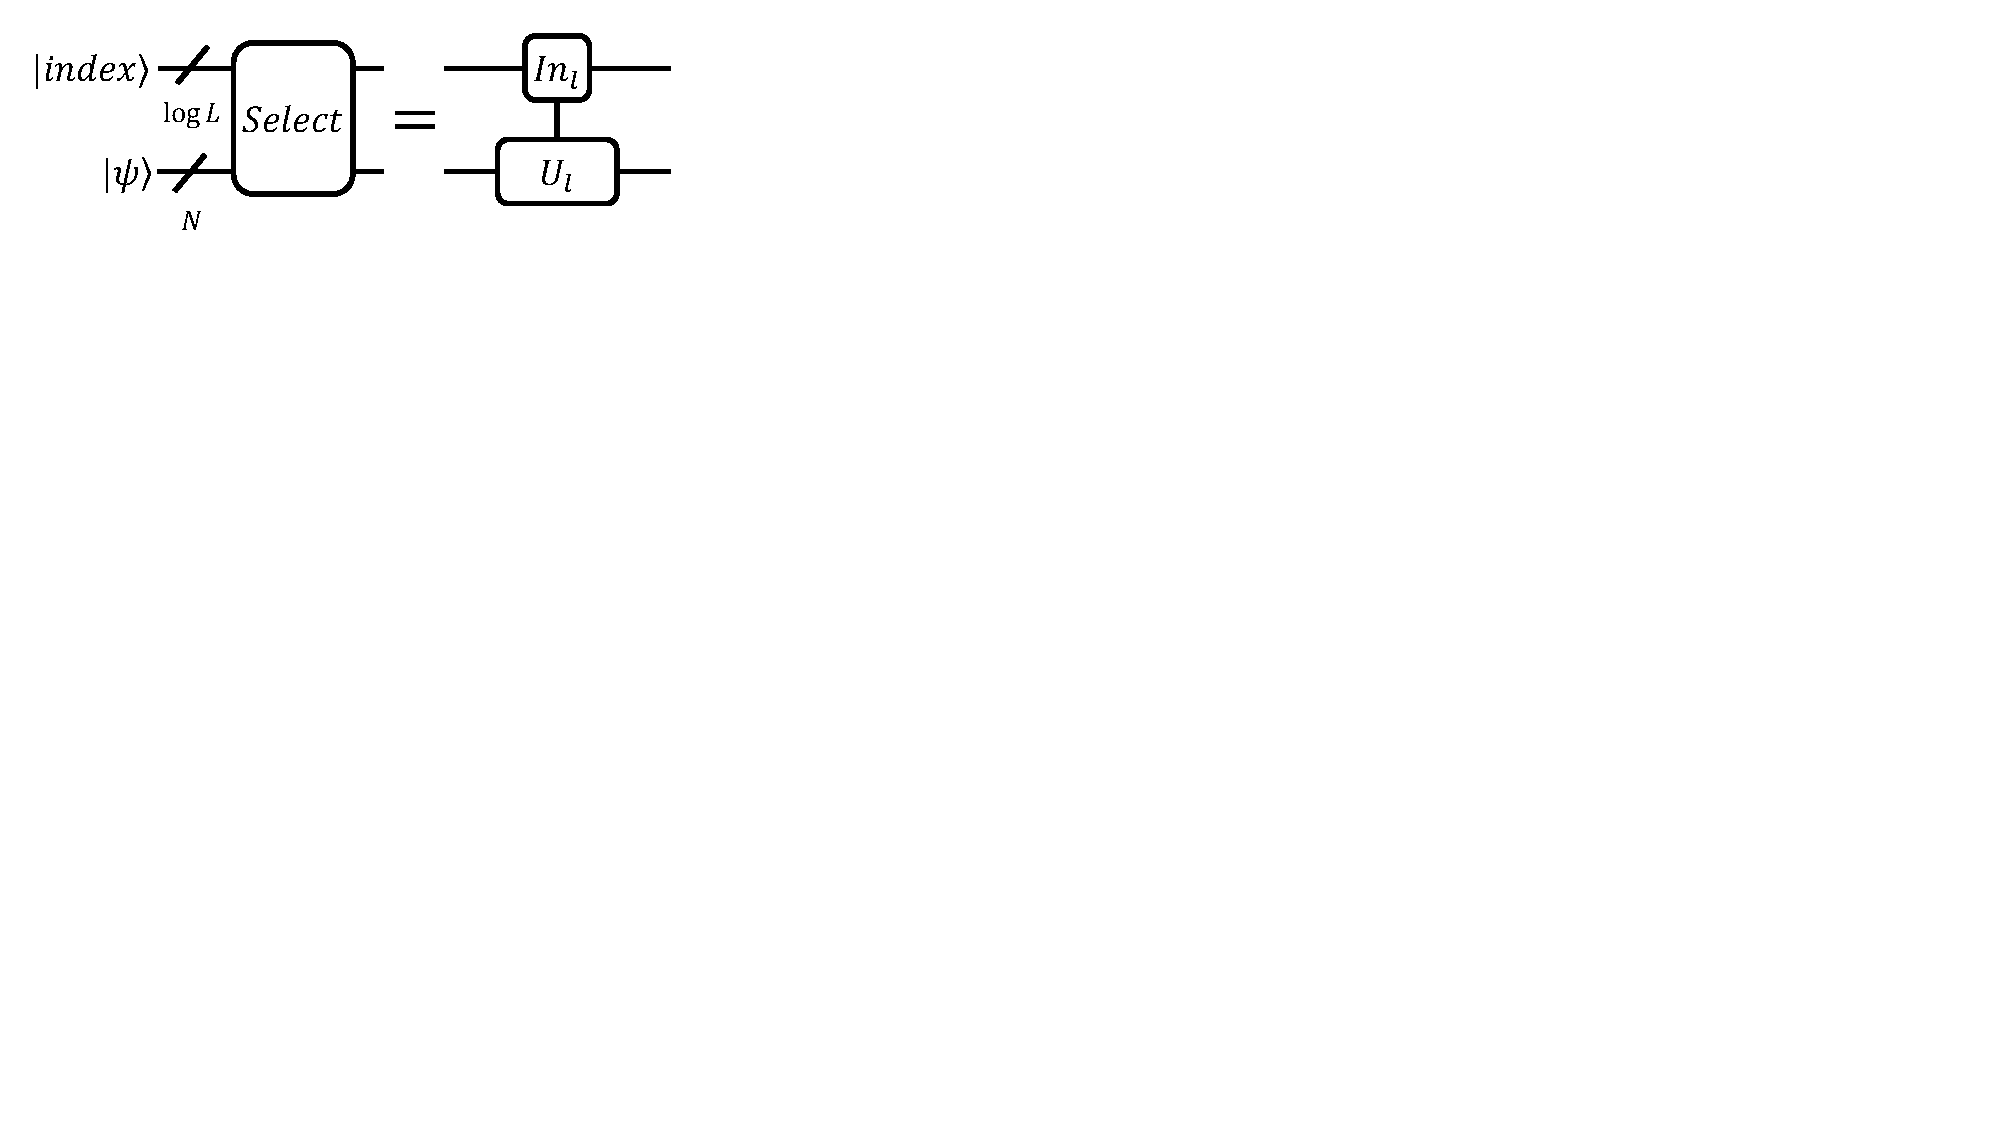
\includegraphics[width=6cm]{figures/select-lcu.pdf}
    \caption{
        \textbf{LCU \textit{Select} Oracle}
        A circuit diagram for the \textit{Select} oracle in LCU is shown.
        This is a naive implementation where no structure in the operator is assumed.
        The \textit{Select} oracle applies the $l^\text{th}$ unitary in the LCU (Eq. \ref{eq:lcu}) onto the system when the index register is in the computational basis state $\ket{l}$
        This can be achieved using a set of uniformly controlled operations (right subfigure).
    }
    \label{fig:unstructured-select}
\end{figure}

If structure in the problem is present, the \textit{Select} oracle can be implemented to leverage that structure as is done in \cite{babbush2018encoding}.
Without any assumptions on the structure in $A$, the \textit{Select} oracle can be implemented by the operator:
\begin{equation}
    \label{eq:select-naive}
    \text{Select} = \sum_{l=0}^{L-1} \ket{l}\bra{l} \otimes U_l
\end{equation}
Similar to the $O_A$ and $O_c$ oracles, the \textit{Select} oracle serially controls upon the computational basis states of the index register and this control structure can be grouped together as a uniformly controlled operation which is discussd in more detail in Appendix \ref{sec:uniformly-controlled-operations}.
This is shown in Figure \ref{fig:unstructured-select}.

As a quick aside, if the implementation of the \textit{Select} oracle is self-inverse, then the LCU block-encoding is also self-inverse.
This structure makes LCU block-encodings particularly well-suited for being applied in algorithms based on Qubitization \cite{low2019hamiltonian}.
Using the construction for \textit{Select} in Eq. \ref{eq:select-naive}, the implementation will be self-inverse if the unitaries themselves are self-inverse.
As an example, this is the case for when the operator $A$ is decomposed in the Pauli basis as the Paulis are self-inverse. 

\subsection{Linear Combination of Operators}
\label{subsec:unification}

LCU block-encodings provide better rescaling factors, yet there are clearly parallels between the $O_A$ oracle and the \textit{Prepare} oracle, as well as the $O_c$ oracle and the \textit{Select} oracle.
Therefore one might ask if we can construct LCU-style block-encodings for a linear combination of \textit{operators} under the assumption that we have access to block-encodings of each operator:
\begin{equation}
    \label{eq:lco}
    A = \sum_{l=0}^{L-1} \alpha_l O_l
\end{equation}
where the $O_l$ are operators and we again restrict the coefficients $\alpha_l$ to be real-valued for simplicity, yet the same strategies to apply operators with imaginary or complex-valued coefficients used for an LCU can be applied here.
% We also restrict the spectral norms of the operators to satisfy $|\bar{O}_l| \leq 1$ for simplicity and note that we can rescale any operator to satisfy this condition and let the rescaling factor be absorbed by the corresponding coefficient.
% However, we note that extra care must be taken when absorbing these rescaling factors such that the rescaling of the linear combination is consistent across all terms.

Another way to frame this is creating an LCU block-encoding where the unitary operators themselves are block-encodings of operators which is described in Section 4.3 of Gilyén et. al \cite{gilyen2019quantum} and noted by Jennings et. al \cite{jennings2023efficient}.
We will refer to this method of block-encoding as an LCO block-encoding (Linear Combination of Operators).
As noted by Jennings et. al \cite{jennings2023efficient} it may be enlightening to consider an LCU block-encoding as a apecial case of an LCO block-encoding wherein the operators in the linear combination are all unitary.

\begin{theorem}
    \label{th:lco}
    Given a matrix $A$ defined by Eq. \ref{eq:lco} and unitary operators $U_l$ that each block-encode the operators $O_l$:
    \begin{equation}
        \label{eq:applying-operator}
        U_l \ket{\psi}\ket{0}_\text{anc} = \bar{O}_l \ket{\psi} \ket{0}_\text{anc} + \beta_{\psi, l} \ket{\perp}
    \end{equation}
    with rescaling factors $\lambda_l$ such that $\lambda_l \bar{O}_l = O_l$.
    
    Define the \textbf{Prepare} oralce by:
    \begin{equation}
        \label{eq:prep-lco}
        \textbf{Prepare}\text{:} \ket{0^{\otimes \lceil \log_2 L \rceil}}_\text{index} \rightarrow \sum_{l=0}^{L-1} \sqrt{| \bar{\alpha}_l | / \lambda} \ket{l}_\text{index}
    \end{equation}
    where $\bar{\alpha_l}$ is given by:
    \begin{equation}
        \label{eq:rescaled-coeffs}
        \bar{\alpha_l} = \frac{\alpha_l \lambda_l}{\max_{l^\prime}{\lambda_{l^\prime}}}
    \end{equation}
    and $\lambda$ is given by:
    \begin{equation}
        \lambda = \sum_{l=0}^{L-1} \bar{\alpha_l}
    \end{equation}

    Define the \textbf{Select} oracle by:
    \begin{equation}
        \label{eq:select-conditions-lco}
        \textbf{Select}\text{:} 
        \begin{cases} 
            \text{Apply $U_l$ on $\ket{\psi}\ket{0}_\text{anc}$} & \text{when $\ket{\text{index}}$ is $\ket{l}$} \\
            \text{Undefined} & \text{Otherwise} \\
        \end{cases}
    \end{equation}
    where the \textbf{Select} oracle applies a block-encoding of $O_l$ on the system register using an additional ancilla register when the index register is in the computational basis state $\ket{l}$ and the action is not strictly defined for other states of the index register.

    Then a block-encoding for $A$ is given by:
    \begin{equation}
        \label{eq:lco-be}
        U_A = (\textbf{Prepare}^\dagger) (\textbf{Select}) (\textbf{Prepare})
    \end{equation}
    with a rescaling factor of:
    \begin{equation}
        \lambda_\text{LCO} = \big(\max_{l}{\lambda_l}\big) \sum_{l=0}^{L-1} | \bar{\alpha}_l | = \sum_{l=0}^{L-1} |\alpha_l \lambda_l|
    \end{equation}
\end{theorem}
The proof that $U_A$ block-encodes $A$ follows from the same proof for LCU block-encodings given by Lin et. al \cite{lin2022lecture}.

To motivate that this rescaling factor is more favorable than a Sparse-Oracle block-encoding, consider the case of the pairing Hamiltonian.
Using the construction given by Liu et. al, the rescaling factor for $H$ is given by:
\begin{equation}
    \lambda_\text{SO}^H = 2^{\lceil \log_2 L \rceil} \max_{ij} |h_{ij}|
\end{equation}
Since each operator in Eq. \ref{eq:pairing-ham} has a spectral norm of $1$, then the rescaling for an LCO block-encoding is simply given by:
\begin{equation}
    \lambda_\text{LCO}^H = \sum_{ij} |h_{ij}|
\end{equation}
and the proof that $\lambda_\text{LCO}^H \leq \lambda_\text{SO}^H$ follows directly from the proof given in Appendix \ref{sec:proof-of-rescaling-factors}.

Implementing the LCO \textit{Prepare} and \textit{Select} oracles can be done similarly to the LCU oracles.
The \textit{Prepare} oracle follows directly from LCU using the rescaled coefficients $\{\bar{\alpha}_l\}$ defined by Eq. \ref{eq:rescaled-coeffs}. 
If structure among the coefficients is present, then this structure can be exploited. 
If no structure exists, then the Grover-Rudolph algorithm can be applied.

The construction for \textit{Select} can again leverage the problem structure if such a structure exists, or it can be generated using uniformly controlled operations following:
\begin{equation}
    \label{eq:select-lco}
    \text{Select} = \sum_{l=0}^{L-1} \ket{l}\bra{l} \otimes U_l
\end{equation}
where the block-encodings for the operators $O_l$ can be constructed using any of the frameworks discussed here.